%%%% Paramétrage du cours %%%%
\def\xxactivite{Cours}
\def\xxauteur{\textsl{Xavier Pessoles}}

\fichefalse
\proftrue
\tdfalse
\courstrue

\def\xxnumchapitre{Chapitre 3 \vspace{.2cm}}
\def\xxchapitre{\hspace{.12cm} Introduction aux réseaux de neurones}

\def\xxcompetences{%
\textsl{%
\textbf{Savoirs et compétences :}\\
\begin{itemize}[label=\ding{112},font=\color{ocre}] 
\item Analyser les principes d'intelligence artificielle.
\begin{itemize}
%\item Régression et classification, apprentissages supervisé et non supervisé.
\item Phases d'apprentissage et d'inférence.
%\item Modèle linéaire monovariable ou multivariable.
\item Réseaux de neurones (couches d'entrée, cachées et de sortie, neurones, biais, poids et fonction d'activation).
\end{itemize}
%\item Interpréter et vérifier la cohérence des résultats obtenus expérimentalement, analytiquement : Ordre de grandeur. Matrice de confusion (tableau de contingence), sensibilité et spécificité d'un test.
\item Résoudre un problème en utilisant une solution d'intelligence artificielle : 
\begin{itemize}
\item Apprentissage supervisé.
\item Choix des données d'apprentissage. 
\item Mise en œuvre des algorithmes (réseaux de neurones).
\item Phases d'apprentissage et d'inférence.
\end{itemize}
\end{itemize}
}}




\def\xxfigures{
%\includegraphics[width=0.6\textwidth]{lola}\\
%\textit{Robot humanoïde Lola}

}%figues de la page de garde%figues de la page de garde

\input{\repStyle/new_pagegarde}
\vspace{2cm}
\pagestyle{fancy}
\thispagestyle{plain}



\section{Introduction}

\subsection{Bref historique}
Dans les années 40, les chercheurs tentent de fabriquer une machine capable d'apprendre à partir de données fournies, de mémoriser des informations et de traiter des informations incomplètes. Pour cela, ils essayent de réaliser des modèles mathématiques de neurones biologiques. S'en suit alors la naissance des premiers modèles de perceptrons. 

L'apprentissage automatisé va alors connaître des hauts et des bas, au gré des avancées scientifiques et technologiques. Dans les années 60, un des premiers coups d'arrêt fût provoqué par la non-capacité des réseaux de neurones à traiter des problèmes non linéaires. Dans les années 80, la rétroproagation du gradient fut proposée. Mais devant le manque de capacité des ordinateurs, la recherche marquât un second coup d'arrêt. Dans les années 90/2000, l'apparition des réseaux convolutifs et leur capacité à analyser les données des images relançât alors les recherches dans ce domaine.

\subsection{Exemples d'applications des réseaux de neurones}
\url{https://fr.wikiversity.org/}
\begin{itemize}
\item Banque	 : prêts et scoring.
\item Cartes de crédit	: détection des fraudes.
\item Finance	 : analyse d'investissements et de fluctuations des taux de change.
\item Assurance : couverture assurantielle et estimation des réserves.
\item Marketing : ciblage des prospections, mesures et comparaisons des campagnes et des méthodes.
\item Archéologie	 : identification et datation de fossiles et d'ossements.
\item Défense : identification de cibles.
\item Environnement : prévisions de la qualité de l'air et de l'eau.
\item Production : contrôles qualité.
\item Médecine : diagnostics médicaux.
\item Energies : estimations des réserves, prévisions de prix.
\item Pharmacie : efficacité de nouveaux médicaments.
\item Psychologie	: prévisions comportementales.
\item Immobilier : études de marchés.
\item Recherche scientifique : identification de spécimens, séquençages de protéines.
\item Télécommunication : détection des pannes de réseaux.
\item Transport : maintenance des voies.
\end{itemize}

\section{Le neurone, les réseaux de neurones}

\subsection{Modèle de neurone}

\begin{defi}{Neurone (ou perceptron)}~\\


\begin{minipage}[c]{.55\linewidth}
Prenons la représentation suivante pour un neurone. On note :
\begin{itemize}
\item $\mathbf{X}$ le vecteur d'entrée et $x_i$ les données de la couche d'entrée;
\item $w_i$ les poids (poids synaptiques);
\item $b$ le biais;
\item $z_0$ la somme pondérée des entrée;
\item $f$ une fonction d'activation; 
\item $\tilde{y}_0$ : la valeur de sortie du neurone.
\end{itemize}
\end{minipage}
\hfill
\begin{minipage}[c]{.4\linewidth}
\begin{center}
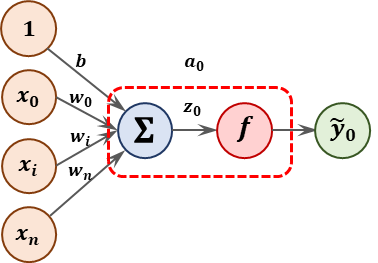
\includegraphics[width=.9\linewidth]{fig_01}
\end{center}
\end{minipage}

On a donc, dans un premier temps  :
$$z_0 = b+ \sum\limits_{i=0}^{n} w_i x_i. $$

Après la fonction d'activation, on a donc en sortie du neurone :
$$\tilde{y}_0 = f(z_0)=f \left( b+ \sum\limits_{i=0}^{n} w_i x_i\right).$$

\begin{rem}
\begin{enumerate}
\item La notation tilde ($\tilde{y}_0$) vient du fait que la valeur de sortie d'une neurone est une valeur estimée qu'il faudra comparer à ${y}_0$ valeur de l'étiquette utilisée pour l'apprentissage supervisé.
\item Par la suite, dans la représentation graphique on ne fera pas apparaître la somme pondérée et la fonction d'activation, mais seulement la valeur de sortie du neurone (notée par exemple $a_0$).
\end{enumerate}
\end{rem}

\end{defi}




\begin{defi}{Fonction d'activation}

Les fonctions d'activation sont des fonctions mathématiques appliquées au signal de sortie ($z$). Il est alors possible d'ajouter des non linéarités à la somme pondérée. On donne ci-dessous quelques fonctions usuelles : 

\begin{center}
\begin{tabular}{|c|c|c|c|}
\hline 
Identité & Heaviside & Logistique & Unité de rectification \\
  &  & (sigmoïde) &  linéaire (ReLU) \\
\hline 
&&&\\
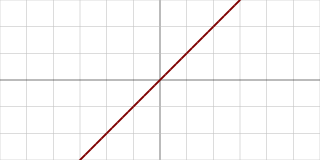
\includegraphics[width=2cm]{fig_03_Identite} &
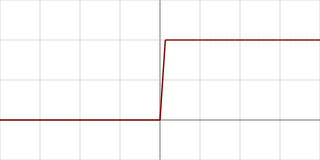
\includegraphics[width=2cm]{fig_03_heaviside} &
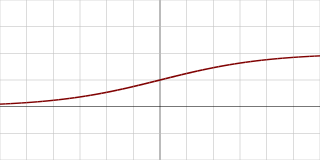
\includegraphics[width=2cm]{fig_03_Logistique} &
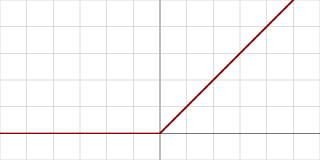
\includegraphics[width=2cm]{fig_03_ReLU} \\
&&&\\
$f(x)=x$ & 
$f(x)=\left\{
\begin{array}{l} 
0 \text{ si } x<0 \\ 1 \text{ si } x \geq 0 \\
 \end{array}\right. $
&
$ f(x) = \dfrac{1}{1+\text{e}^{-x}}$ &
$f(x)=\left\{
\begin{array}{l} 
0 \text{ si } x<0 \\ x \text{ si } x \geq 0 \\
 \end{array}\right. $ \\
\hline 
\end{tabular}
\end{center}

\end{defi}


\begin{rem}
Influence des poids et des biais sur la sortie du perceptron en utilisant une fonction d'activation ReLU.

\begin{minipage}[c]{.45\linewidth}
\begin{center}
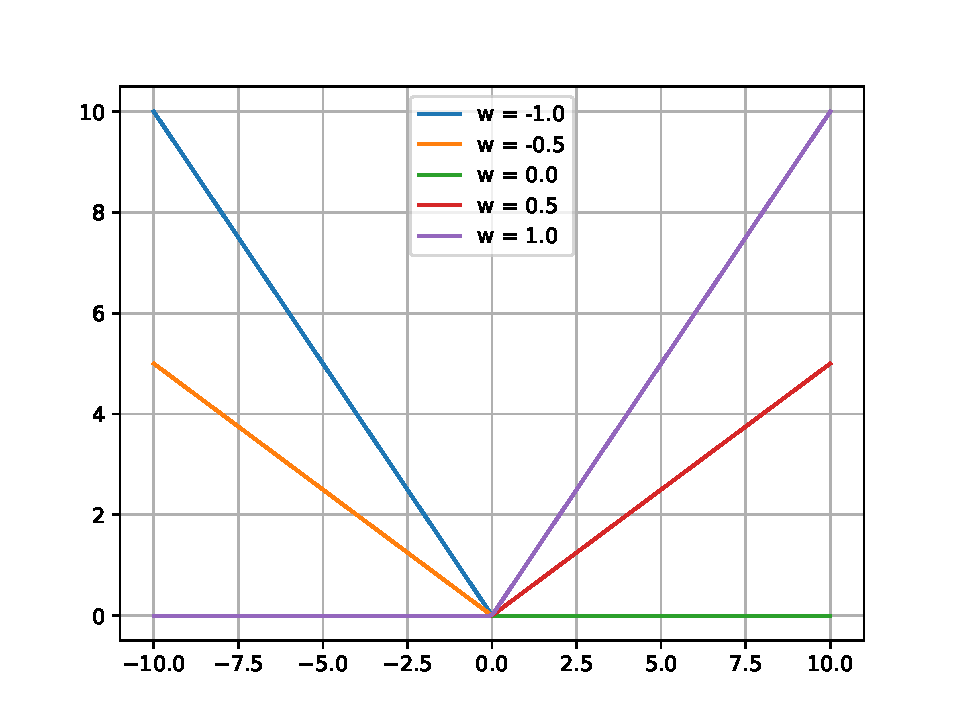
\includegraphics[width=.9\linewidth]{poids}
\end{center}
\end{minipage}
\hfill
\begin{minipage}[c]{.45\linewidth}
\begin{center}
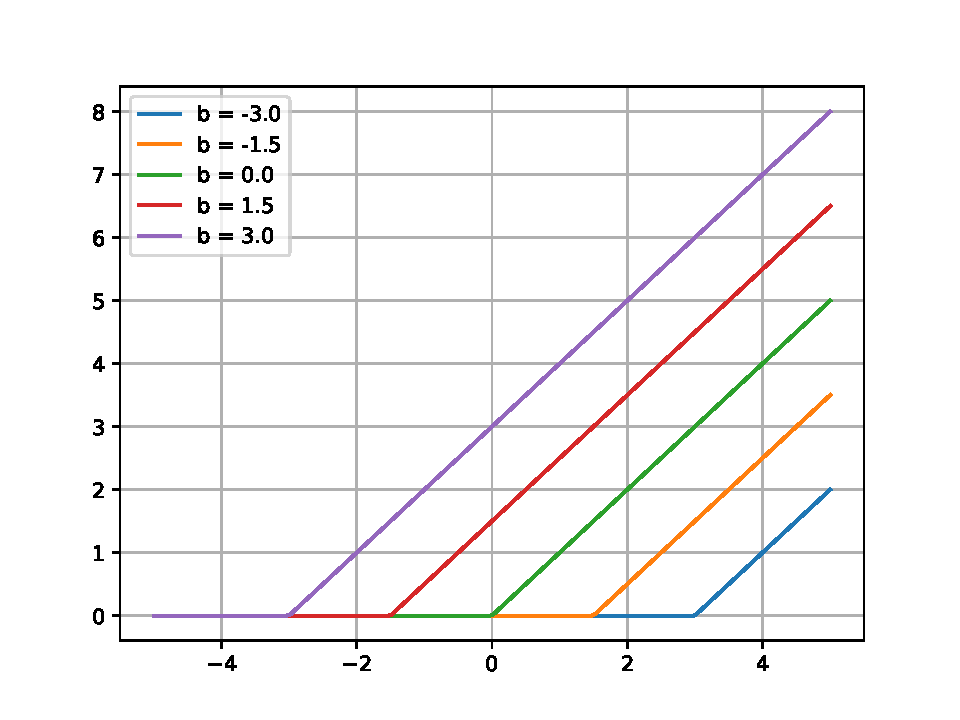
\includegraphics[width=.9\linewidth]{biais}
\end{center}
\end{minipage}

On peut ainsi voir qu'avec la fonction d'activation ReLU, plus le poids sera grand en valeur absolu, plus la neurone amplifiera le signal d'entrée. 

Le biais permettra de prendre en compte le << niveau >> du signal d'entrée à partir duquel, le signal doit être amplifié, ou non.

\end{rem}


\begin{exemple}~\\



\begin{minipage}[c]{.4\linewidth}

Prenons un neurone à deux entrées binaires. 
Initialisation les poids et le biais avec des valeurs aléatoires : $w_0 = -0,3$, $w_1 = 0,8$ et $b=0,2$.

\begin{center}
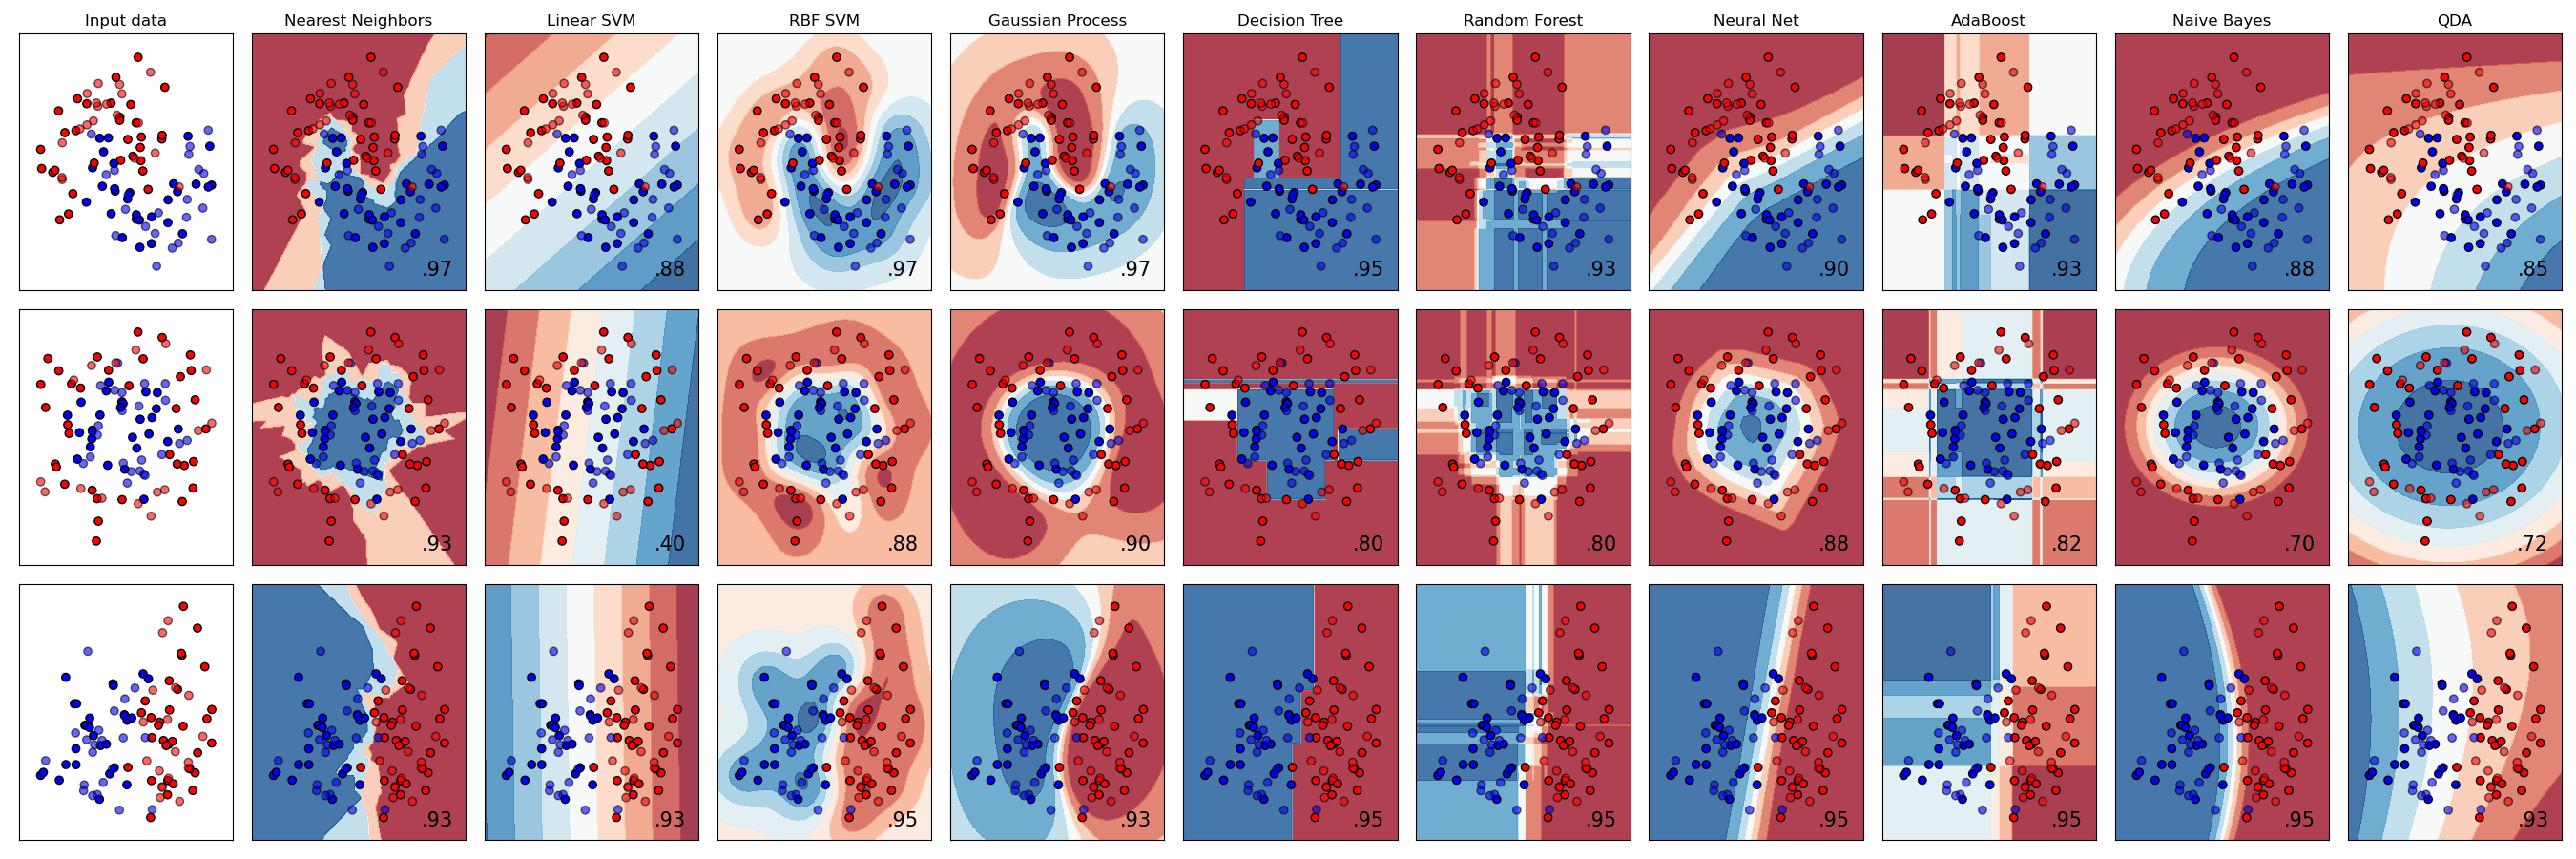
\includegraphics[width=.9\linewidth]{fig_02}
\end{center}
\hfill
\end{minipage}
\begin{minipage}[c]{.55\linewidth}


On peut donc évaluer l'ensemble des sorties calculable par le neurone.

\begin{center}
\begin{tabular}{|c|c|| c || c| c|c|c|}
\hline
$x_0$ & $x_1$ & $z$ & Id. & H. & Sig. & ReLu \\
\hline
\hline
0 & 0 & 0,2   &   0,2   &  1 & 0.549 & 0,2 \\
0 & 1 & 1     &    1     &  1 & 0.731  & 1\\
1 & 0 & -0.1  &    -0.1 &  0 &0.475 & 0 \\
1 & 1 & 0.7  &     0.7  &  1 &0.668 & 0.7\\
\hline
\end{tabular}
\end{center}
\end{minipage}

\end{exemple}


\section{Réseaux de neurones}
\url{https://playground.tensorflow.org/}
%LSTM


\subsection{Modélisation d'un réseau de neurones} 

\begin{defi}{Couches} 

Un réseau de neurones est un ensemble de neurones reliés, par couches, entre eux. 

Dans un réseau de neurones \textbf{dense} tous les neurones de la couche $i$ seront reliés à tous les neurones de la couche $i+1$.

\begin{itemize}
\item Couche d'entrée : cette couche est une copie de l'ensemble des données d'entrées. Le nombre de neurones de cette couche correspond donc aux nombre de données d'entrées. On note $\mathbf{X} = \left( x_0, ..., x_n\right)$ le vecteur d'entrées.
\item Couche cachée (ou couche intermédiaire) : il s'agit d'une couche qui a une utilité intrinsèque au réseau de neurones. Ajouter des neurone dans cette couche (ou ces couches) permet donc d'ajouter de nouveaux paramètres.  Pour une couche, la même fonction d'activation est utilisée pour tous les neurones. En revanche la fonction d'activation utilisée peut être différente pour deux couches différentes. Les fonctions d'activations des couches intermédiaires sont souvent non linéaires.
\item Couche de sortie : le nombre de neurones de cette couche correspond au nombre de sorties attendues. La fonction d'activation de la couche de sortie est souvent linéaire. On note $\mathbf{Y} = \left( y_0, ..., y_y\right)$ le vecteur des sorties.
\end{itemize}
%\begin{minipage}[c]{.5\linewidth}
\begin{center}
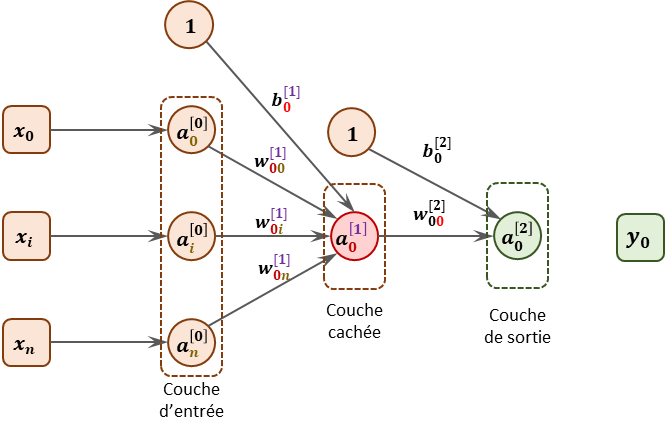
\includegraphics[width=.8\linewidth]{fig_04}
\end{center}
%\end{minipage}

En utilisant la loi de comportement du modèle de perceptron, on peut donc exprimer $\mathbf{Y}=\mathcal{F}\left(\mathbf{X}\right)$ 
où $\mathcal{F}$ est une fonction dépendant des entrées, des poids et des biais.


Notations : 
\begin{itemize}
\item on note $w^{[\ell]}_{jk}$ les poids permettant d'aller vers la couche $\ell$ depuis le neurone $k$ vers le neurone $j$;
\item $b^{[\ell]}_{j}$ le biais permettant d'aller sur le neurone $j$ de la couche $\ell$;
\item $f^{[\ell]}$ la fonction d'activation de la couche $\ell$;
\item $n^{[\ell]}$ le nombre de neurones de la couche $\ell$.
\end{itemize}
\end{defi}

\begin{defi}{Équation de propagation}

Pour chacun des neurones $a_j^{[\ell]}$ on peut donc écrire l'équation de propagation qui lui est associé : 
$$
a_j^{[\ell]} = f^{[\ell]}\left(\sum\limits_{k=0}^{n^{[\ell-1]}}\left( w^{[\ell]}_{jk} a_k^{[\ell-1]} \right) + b^{[\ell]}_{j}\right) = f^{[\ell]}\left(z_j^{[\ell]}\right).
$$

\end{defi}


\begin{exemple}~\\

\begin{minipage}[c]{.4\linewidth}

Prenons un réseau de neurones à 3 couches : 
\begin{itemize}
\item 1 couche d'entrée à 2 neurones;
\item 1 couche cachée à 2 neurones, de fonction d'activation $f_1$;
\item 1 couche de sortie à 1 neurone, de fonction d'activation $f_2$; 
\end{itemize}

Initialisation les poids et le biais avec des valeurs aléatoires : $w_0 = -0,3$, $w_1 = 0,8$ et $b=0,2$.



\end{minipage}\hfill
\begin{minipage}[c]{.55\linewidth}
\begin{center}
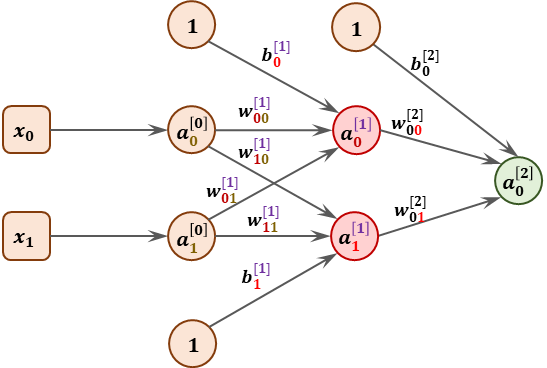
\includegraphics[width=.9\linewidth]{fig_05}
\end{center}
%On peut donc évaluer l'ensemble des sorties calculable par le neurone.
%
%\begin{center}
%\begin{tabular}{|c|c|| c || c| c|c|c|}
%\hline
%$x_0$ & $x_1$ & $z$ & Id. & H. & Sig. & ReLu \\
%\hline
%\hline
%0 & 0 & 0,2   &   0,2   &  1 & 0.549 & 0,2 \\
%0 & 1 & 1     &    1     &  1 & 0.731  & 1\\
%1 & 0 & -0.1  &    -0.1 &  0 &0.475 & 0 \\
%1 & 1 & 0.7  &     0.7  &  1 &0.668 & 0.7\\
%\hline
%\end{tabular}
%\end{center}
\end{minipage}

Il est possible d'écrire que 
$y_0 = a_0^{[1]}$ 
$ = f_2\left(b_0^{[2]}+ w_{00}^{[2]} a_0^{[1]}+ w_{01}^{[2]} a_1^{[1]}\right)$.

Par ailleurs : 
 $  a_0^{[1]}$ 
$ = f_1\left(b_0^{[1]}+ w_{00}^{[1]} a_0^{[0]}+ w_{01}^{[1]} a_1^{[0]}\right)$ et
  $  a_1^{[1]}$ 
$ = f_1\left(b_1^{[1]}+ w_{10}^{[1]} a_0^{[0]}+ w_{11}^{[1]} a_1^{[0]}\right)$.

Au final, on a donc 

$y_0 = a_0^{[1]}$
$ =  f_2\left(b_0^{[2]}+ w_{00}^{[2]}\left(f_1\left(b_0^{[1]}+ w_{00}^{[1]} a_0^{[0]}+ w_{01}^{[1]} a_1^{[0]}\right)\right)+ w_{01}^{[2]} \left( f_1\left(b_1^{[1]}+ w_{10}^{[1]} a_0^{[0]}+ w_{11}^{[1]} a_1^{[0]}\right)\right)\right) $ 


\end{exemple}

\begin{defi}{Paramètres}

Les paramètres du réseau de neurones sont les poids et les biais, autant de valeurs que l’entraînement devra déterminer.

\end{defi}
\begin{methode}{Calcul du nombre de paramètres -- à vérifier} ~\\

Soit un jeu de données étiquetées avec $n$ entrées et $p$ sorties.

On construit un réseau possédant $\ell$ couches  et $a_\ell$ le nombre de neurones de la couche  $\ell$. Dans ce cas, la première couche est la couche d'entrée ($a_1 = n$) et la dernière couche et la couche de sortie ($a_\ell= p$).


\textbf{Nombre de poids :} $n_w = \sum\limits_{i=1}^{\ell-1} \left(a_i \times a_{i+1}\right)$.

\textbf{Nombre de bais :} $n_b = \sum\limits_{i=2}^{\ell}\left( a_i  \right)$.


Au final, le nombre total de paramètre à calculer est donné par $N=n_w+n_b$.

\end{methode}
\begin{obj}
Soit un jeu de données étiquetées. On note $\mathbf{X}$ le vecteur des données d'entrées. On note $\mathbf{Y}$ le vecteur des données de sorties. On note
$\mathbf{\tilde{Y}}$ le vecteur de sortie calculé par le réseau de neurones.


L'objectif de la phase d'apprentissage du réseau de neurones est de déterminer les valeurs de  l'ensemble des poids et des biais de telle sorte que l'écart entre $\mathbf{Y}$ 
et $\mathbf{\tilde{Y}}$ soit minimale.
\end{obj}




\subsection{Fonction de coût}
Dans le but de minimiser l'écart entre la sortie du réseau de neurones et la valeur réelle de la sortie, on utilise une fonction coût (ou fonction de perte). Il est possible de définir plusieurs types de fonctions, notamment en fonction du type de problème à traiter (classification ou régression par exemple).

\begin{defi}{Fonction coût régression}
Notons $nb$ le nombre de données dans la base d'entraînement. Dans le cadre d'un problème de régression, on peut définir la fonction coût comme la moyenne des erreurs quadratique entre la valeur donnée par l'équation de propagation et la valeur de l'étiquette :
$$
C = \dfrac{1}{nb} \sum \limits_{i=1}^{nb} \left( \mathbf{\tilde{Y_i}} - \mathbf{Y_i}  \right)^2
$$
\end{defi}
\begin{obj}
L'objectif est dès lors de déterminer les poids et les biais qui minimisent la fonction coût.
\end{obj}



\subsection{Notion de rétropropagation -- Descente de gradient}

\begin{minipage}[c]{.55\linewidth}
En réutilisant l'exemple ci-contre, nous allons présenter succinctement comment est minimisée la fonction coût.
Pour cela, il va falloir dériver la fonction coût par rapport à chacune des variables. 

Cherchons uniquement à déterminer le coût que par rapport à un seul vecteur d'entrée du jeu d'entraînement. On a alors : 
\begin{itemize}
\item $C = \left( \mathbf{\tilde{Y_i}} - \mathbf{Y_i}  \right)^2$ $= \left( a^{[2]}_{0} - y  \right)^2$;
\item $ a^{[2]}_{0} = f^{[2]}\left(z_0^{[2]}\right)$;
\item $z_0^{[2]} =\sum\limits_{k=0}^{1}\left( w^{[2]}_{0k} a_k^{[1]} \right) + b^{[2]}_{0}$.
\end{itemize}

\end{minipage}\hfill
\begin{minipage}[c]{.4\linewidth}
\begin{center}
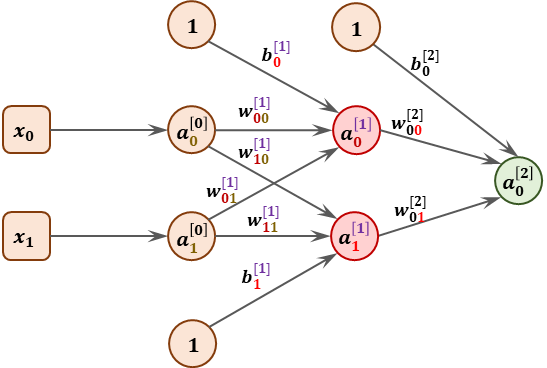
\includegraphics[width=.9\linewidth]{fig_05}
\end{center}
%On peut donc évaluer l'ensemble des sorties calculable par le neurone.
%
%\begin{center}
%\begin{tabular}{|c|c|| c || c| c|c|c|}
%\hline
%$x_0$ & $x_1$ & $z$ & Id. & H. & Sig. & ReLu \\
%\hline
%\hline
%0 & 0 & 0,2   &   0,2   &  1 & 0.549 & 0,2 \\
%0 & 1 & 1     &    1     &  1 & 0.731  & 1\\
%1 & 0 & -0.1  &    -0.1 &  0 &0.475 & 0 \\
%1 & 1 & 0.7  &     0.7  &  1 &0.668 & 0.7\\
%\hline
%\end{tabular}
%\end{center}
\end{minipage}


Commençons par déterminer la dérivée partielle par rapport à un poids de la couche de sortie : 

$\dfrac{\partial C}{\partial w^{[2]}_{00}}=\dfrac{\partial C}{\partial a^{[2]}_{0}}\dfrac{\partial  a^{[2]}_{0}}{\partial z^{[2]}_{0}}\dfrac{\partial z^{[2]}_{0}}{\partial w^{[2]}_{00}}$.

De même, on peut calculer la dérivée partielle du coût par rapport au biais : 
$\dfrac{\partial C}{\partial b^{[2]}_{0}}=\dfrac{\partial C}{\partial a^{[2]}_{0}}\dfrac{\partial  a^{[2]}_{0}}{\partial z^{[2]}_{0}}\dfrac{\partial z^{[2]}_{0}}{\partial b^{[2]}_{0}}$.

Calculons les dérivées nécessaires : 
\begin{multicols}{4}
\begin{itemize}
\item $\dfrac{\partial C}{\partial a^{[2]}_{0}}$ $= 2\left( a^{[2]}_{0} - y  \right)$;
\item $ \dfrac{\partial  a^{[2]}_{0}}{\partial z^{[2]}_{0}} = f'^{[2]}\left(z_0^{[2]}\right)$;
\item $\dfrac{\partial z^{[2]}_{0}}{\partial w^{[2]}_{00}}  = a_0^{[1]} $.
\item $\dfrac{\partial z^{[2]}_{0}}{\partial b^{[2]}_{0}} = 1$.
\end{itemize}
\end{multicols}

On a donc, 
$\dfrac{\partial C}{\partial w^{[2]}_{00}} = 2\left( a^{[2]}_{0} - y  \right)  f'^{[2]}\left(z_0^{[2]}\right) a_0^{[1]}$
et 
$\dfrac{\partial C}{\partial b^{[2]}_{0}} = 2\left( a^{[2]}_{0} - y  \right)  f'^{[2]}\left(z_0^{[2]}\right) $.

Prenons le cas ou la fonction d'activation est la fonction identité. 
On a alors
$\dfrac{\partial C}{\partial w^{[2]}_{00}} = 2\left( a^{[2]}_{0} - y  \right)   a_0^{[1]}$
et 
$\dfrac{\partial C}{\partial b^{[2]}_{0}} = 2\left( a^{[2]}_{0} - y  \right)   $...

On va ainsi pouvoir exprimer $\dfrac{\partial C}{\partial w^{[2]}_{00}}$, $\dfrac{\partial C}{\partial w^{[2]}_{01}}$ , $\dfrac{\partial C}{\partial b^{[2]}_{0}}$, ... 
On pourrait ici écrire 9 équations en fonction des différents poids, des biais et des entrées $x_0$ et $x_1$.  

\`A partir de cela, on va modifier les poids comme suit : 
\begin{itemize}
\item $ w^{[2]}_{00,i+1}=w^{[2]}_{00,i}-\eta  \dfrac{\partial C}{\partial w^{[2]}_{00,i}}$;
\item $ b^{[2]}_{0,i+1}=b^{[2]}_{0,i}-\eta  \dfrac{\partial C}{\partial b^{[2]}_{0,i}}$.
\end{itemize}

On réitère ensuite les opérations précédentes jusqu'à ce que la fonction coût ait été suffisamment réduite.

\begin{defi}{Taux d'apprentissage}
On définit l'hyperparamètre $\eta\in[0,1[$ comme étant le taux d'apprentissage. Si ce taux d'apprentissage est très grand, l'algorithme d'apprentissage mettra beaucoup de temps à trouver le minimum. S'il est trop grand, le minimum peut ne jamais être trouvé. 

\end{defi}


\begin{defi}{Gradient}
Dés lors, dans le cas présenté, on peut définir le gradient comme le vecteur
$\text{grad} C = \begin{bmatrix}
\dfrac{\partial C}{w^{[1]}_{}} \\
\dfrac{\partial C}{b^{[1]}_{}} \\
\vdots
\\
\dfrac{\partial C}{w^{[l]}_{}} \\
\dfrac{\partial C}{b^{[l]}_{}} \\

\end{bmatrix}
$.


\end{defi}

\subsection{Fin d'apprentissage}

\begin{defi}{Epoch}
On appelle \textit{epoch} un cycle d'apprentissage où tous les poids et tous les biais ont été mis à jour en faisant passer toutes les données du jeu d’entraînement dans les algorithmes de propagation et de rétropropagation.
\end{defi}

Les méthodes pour stopper l'apprentissage sont essentiellement empiriques. On pourrait en effet fixer un nombre d'epoch ou une valeur d'erreur admissible et s'arrêter à ce moment là. Dans la pratique, se focaliser sur l'erreur n'est généralement pas satisfaisant. En effet, il y a risque de << suraprentissage >>.

\begin{center}
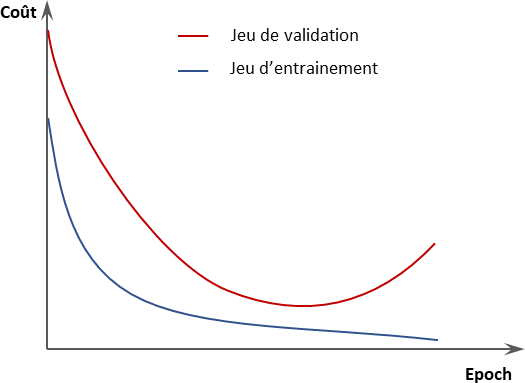
\includegraphics[width=.6\linewidth]{fig_06_overfitting}
\end{center}

Dans la figure suivante, on réalise un entraînement sur le jeu de données (une epoch) à la fin de l'epoch on dispose d'un premier modèle de réseau de neurones.  On détermine alors l'erreur commise en utilisant le jeu d'entraînement puis l'erreur commise sur le jeu de validation.  On calcule ensuite l'erreur commise par le modèle sur le jeu de validation. (On rappelle que le jeu de validation ne sert pas à modifier les poids et les biais.)

On réalise de même à la fin de l'epoch suivante etc...

<< Logiquement >> l'erreur décroît toujours avec le jeu d’entraînement car la descente du gradient a pour objectif de réduire cette erreur. 

Sur le jeu de validation, l'erreur décroît pendant un certain nombre d'epoch puis augmente. 

Il existe en fait un stade à partir duquel le réseau de neurones se spécialise sur le jeu d’entraînement et devient donc incapable de réaliser des prédictions fiables sur un nouveau je de données. On parle de surentraînement (ou d'overfitting).
 
\begin{exemple} \textit{Wikipedia} ~\\
\begin{minipage}[c]{.45\linewidth}
La ligne verte représente un modèle sur-appris et la ligne noire représente un modèle régulier. La ligne verte classifie trop parfaitement les données d’entraînement, elle généralise mal et donnera de mauvaises prévisions futures avec de nouvelles données. Le modèle vert est donc au final moins bon que le noir.
\end{minipage} \hfill
\begin{minipage}[c]{.45\linewidth}
\begin{center}
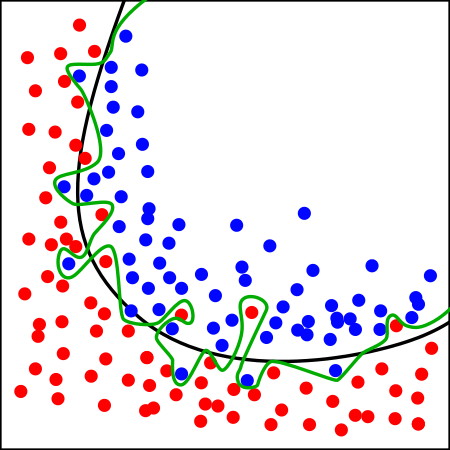
\includegraphics[width=.7\linewidth]{fig_07_overfitting}
\end{center}
\end{minipage} 
\end{exemple}



\section{Pour aller plus loin...}

Les réseaux présentés ci-dessus sont les réseaux dits denses (ou fully-connected). On utilise d'autre types de réseaux pour une meilleure prédiction en fonction des données d'entrées : 
\begin{itemize}
\item réseaux convolutifs (CNN) pour l'analyse d'images;
\item réseaux de neurones récurrents pour les données temporelles \textit{etc..}
\end{itemize}

Le cours suivant présente les réseaux de type NARX et MRAC qui sont utilisés dans Matlab pour gérer les signaux temporels. Ils ont la particularité de réutiliser les sorties estimées par le réseau comme entrées décalées. 

%Exemples : 
%\url{https://makina-corpus.com/blog/metier/2017/initiation-au-machine-learning-avec-python-pratique}

%\begin{thebibliography}{2}
%   \bibitem[1]{ref1} Éric Biernat et Michel Lutz. {\it Data science : fondamentaux et études de cas.} Eyrolles.
%\end{thebibliography}

